\documentclass{article}
\usepackage[swedish]{babel}	
\usepackage[utf8]{inputenc} 		
\usepackage{amsmath} 

\usepackage{fancyhdr}
\usepackage{lastpage}
\usepackage{lineno}
\usepackage{lmodern}
\usepackage[T1]{fontenc}
\usepackage[utf8]{inputenc}
\usepackage[swedish]{babel}
\usepackage{microtype}
\usepackage{systeme}
\usepackage{amsmath,amssymb,amsthm,mathrsfs,latexsym,tikz,url}
\usepackage{epigraph,graphicx}
%\usepackage{titlesec} %For formatting sections
\usepackage{listings}
\usepackage{listingsutf8}
\usepackage{color}
\usepackage{todonotes}
\presetkeys%
    {todonotes}%
    {inline,backgroundcolor=yellow}{}

\graphicspath{ {./}{./figures/} {images/}}
\DeclareGraphicsExtensions{.png,.pdf}

\definecolor{dkgreen}{rgb}{0,0.6,0}
\definecolor{gray}{rgb}{0.5,0.5,0.5}
\definecolor{mauve}{rgb}{0.58,0,0.82}

\lstset{frame=tb,
  language=Python,
  aboveskip=3mm,
  belowskip=3mm,
  showstringspaces=false,
  columns=flexible,
  basicstyle={\small\ttfamily},
  numbers=none,
  numberstyle=\tiny\color{gray},
  keywordstyle=\color{blue},
  commentstyle=\color{dkgreen},
  stringstyle=\color{mauve},
  breaklines=true,
  breakatwhitespace=true,
  tabsize=4
}


\setlength{\parindent}{0.0cm}
\setlength{\parskip}{0.1cm}



\begin{document}


\title{Lab 1 Machine Learning}
\author{Anton Stråhle \& Jan Alexandersson}
\maketitle 

\section*{Assignment 0}

\begin{itemize}
 \item MONK-1: The true concepts of the MONK-1 data set makes learning difficult due to the relation between $a_1$ and $a_2$, meaning we cannot split them up as easily as we would like. 
 \item MONK-2: For this data the true concept indicates that we have relations between all the attibutes $a_k$ which once again makes it troublesome to split the attibutes. Specifically it is difficult to split based on the value of one attribute.
 \item MONK-3: The true concept of MONK-3, as with the previous two data sets, makes learning difficult due to the realtionships between attributes. We also have a smaller sample size as well as $5\%$ white noise which makes further increases the difficulty of learning.
 \end{itemize}
 
 As such we believe that MONK-3 is the most difficult problem to learn.


\section*{Assignment 1}

\begin{center}
 \begin{tabular}{|c | c|} 
 \hline
 Dataset & Entropy  \\ [0.5ex] 
 \hline \hline
 MONK-1 & 1.0 \\ 
 %\hline
 MONK-2 & 0.9571174283 \\ 
 %\hline
 MONK-3 & 0.9998061328 \\ [1ex] 
 \hline
\end{tabular}
\end{center}


\section*{Assignment 2}

Entropy can be described as the level of uncertainity of a random variable. Formally the entropy of a non-negative discrete random variable $X$ is defined as
$$
H(X) = -\sum_{k=0}^{\infty}\mathbb{P}(X=k)\log_2(\mathbb{P}(X=k))
$$

The uncertainity of a uniform distribution will always be higher than that of a non-unifrom distribution which implies that the entropy of a non-uniform distirbution will be smaller than that of a uniform distribution with the same number of outcomes. If we for example have a $n$ different outcomes the entropy of a uniform distribution will always be $\log_2(n)$ whilst the entropy of a non-uniform one will always be strictly less than $\log_2(n)$.


\section*{Assignment 3}

\begin{center}
 \begin{tabular}{|c | c c c c c c |} 
 \hline
 Dataset & A1 & A2 & A3 & A4 & A5 & A6 \\ [0.5ex] 
 \hline \hline
 MONK-1 & 0.07527 & 0.00584 & 0.00471 & 0.02631 & \textcolor{blue}{\textbf{0.28703}} & 0.00076 \\ 
 %\hline
 MONK-2 & 0.00376 & 0.00246 & 0.00106 & 0.01566 & \textcolor{blue}{\textbf{0.01728}} & 0.00625 \\ 
 %\hline
 MONK-3 & 0.00712 & \textcolor{blue}{\textbf{0.29374}} & 0.00083 & 0.00289 & 0.25591 & 0.00708  \\ [1ex] 
 \hline
\end{tabular}
\end{center}


\section*{Assignment 4}

Assuming we have split using the attribute which maximizes the information gain the remaining uncertainity in the subsets $S_k$ will be minimized, meaning that the corresponding entropy of those subsets will in turn also be minimized. 

We wish to make splits such that they minimze the uncertainity within the remaining subsets. By using entropy as the measure of the uncertainity within these subsets the maximization of the information gain corresponds to the minimization of the entropy, and as such also the uncertainity. 

\section*{Assignment 5}


Run the code below for MONK-1 and MONK-3 and their respective testdata to obtain a sample which we can 
compute the mean and variance on.

\begin{center}
 \begin{tabular}{|c | c | c |} 
 \hline
 Dataset & Error(Train) &  Error(Test) \\ [0.5ex] 
 \hline \hline
 MONK-1 & 0.0 & 0.1713 \\ 
 %\hline
 MONK-2 & 0.0 & 0.30787 \\ 
 %\hline
 MONK-3 & 0.0 & 0.05556  \\ [1ex] 
 \hline
\end{tabular}
\end{center}

The training error is $0$ for all three problems since we have constructed complete trees in all cases which overfits the training data, meaning that our models will classifcy the training data perfectly. This overfitting also leads to the high test error rates as the models as the test data and training data are obviously different. 

As can be seen in the table above our assumptions from Assignment 0 were incorrect as we assumed that MONK-3 would present the most difficulties. This does however not seem to be the case since it has the lowest test error of the three data sets. 


\section*{Assignment 6}

We know that the depth of a tree decides both the bias and the variance. A deeper tree will have higher variance but lower bias whilst a more shallow tree has lower variance but higher bias. A more complex tree structure tends to overfit the data and rarely predicts the test data well. By pruning the tree we no longer have the possibility of very specific predictions as for the more complex model, meaning that we have an incrase in bias. What we gain in return is however a smaller variance as any missclassifications deviate less compared to the complex model.

\section*{Assignment 7}

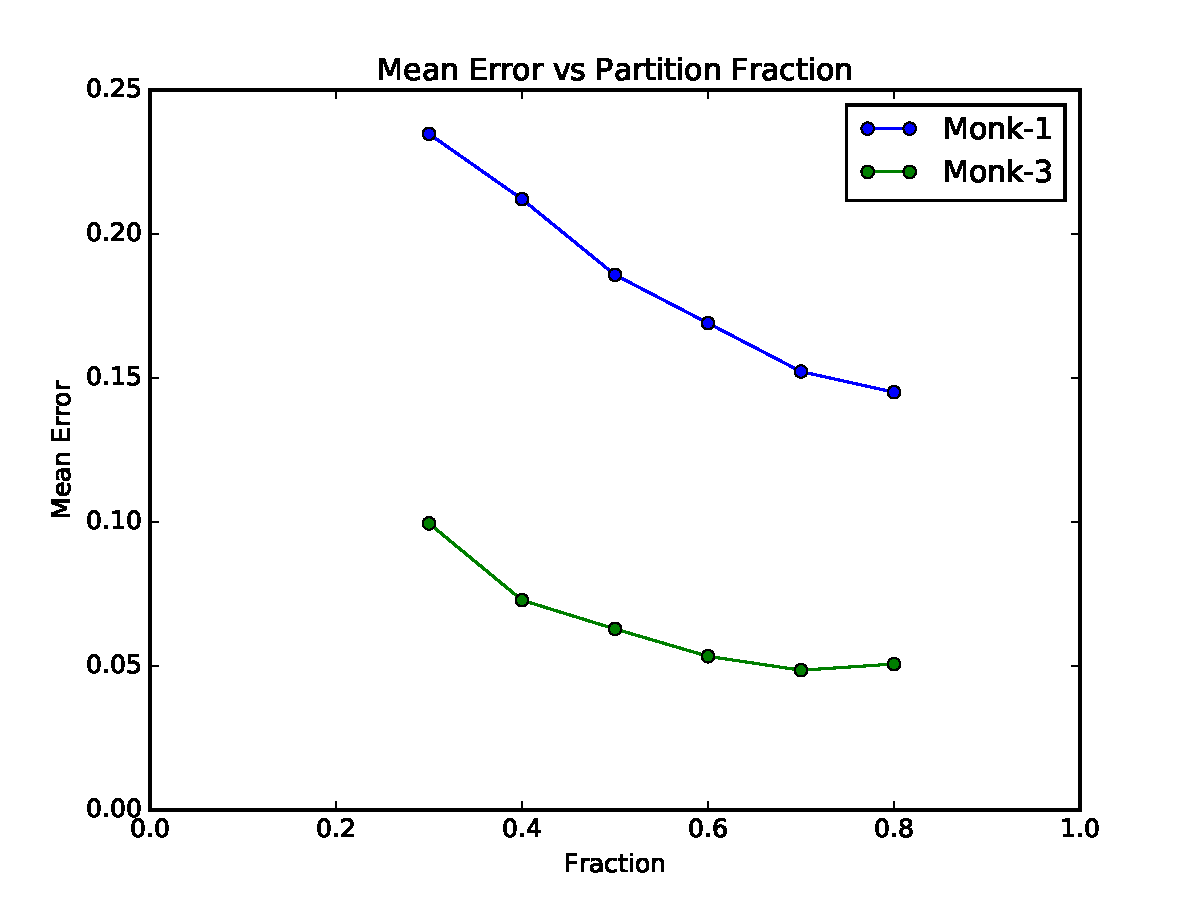
\includegraphics[width = 12cm]{figure_1.pdf}

\begin{center}
 \begin{tabular}{|c c c c c c c|} 
 \hline
 Fraction = & 0.3 & 0.4 & 0.5 & 0.6 & 0.7 & 0.8  \\ [0.5ex] 
 \hline 
 MONK-1 Sd \vline & 0.0436 & 0.0405 & 0.0409 & 0.0432 & 0.0415 & 0.0383 \\ 
 \hline
 MONK-3 Sd  \vline & 0.0578 & 0.0421 & 0.0378 & 0.0322 & 0.0284 & 0.0298 \\ [1ex] 
 \hline
\end{tabular}

It seems as if a split of $(80,20)\%$ reduces the Mean Error for Monk-1. Even though the decrease in Mean Error seems to decrease with the increase of fraction we have to keep in mind that having $100\%$ of the data allocated to training and $0\%$ to validation does in fact lead to an increase in the mean error as we saw in Assignment 5. For MONK-3 the reduction seems to be at $0.7$. We also note that the standard deviation of the mean errors for both MONK-1 and MONK-3 are minimized when using the aforementioned fractions as can be seen in the table above.

\end{center}

\section*{Appendix}

\begin{lstlisting}
def prune(data, test):
	pruned_trees_fraction = []
	for frac in fraction:
		train, val = partition(data, frac)
		t = d.buildTree(train, m.attributes)
		all_pruned = d.allPruned(t)
		
		#I suppose t is included in all_pruned
		best_tree_perf = 0
		for t in all_pruned:
			candidate_perf = d.check(t,val)
			if best_tree_perf < candidate_perf:
				best_tree_perf = candidate_perf
				best_tree = t
		
		pruned_trees_fraction.append(1-d.check(best_tree, test))
	return pruned_trees_fraction
\end{lstlisting}


\end{document}

